\subsection{Comparing with EMV2 Modeling}
\label{subsec:comparison_with_EMV2}
In this section, we use a few examples from the WBS system to illustrate the differences in Safety Annex and EMV2 modeling. The AADL and EMV2 code examples are adapted from ~\cite{WBS_EMV2_Example}.

Below is the AADL component for the command function unit of the Braking and Steering Control Unit (BSCU) in the WBS system, and the error propagations and component error behavior specified in EMV2:

\begin{figure}[h!]
	\hspace*{-4cm}
\vspace{-0.5in} 
\begin{center}
	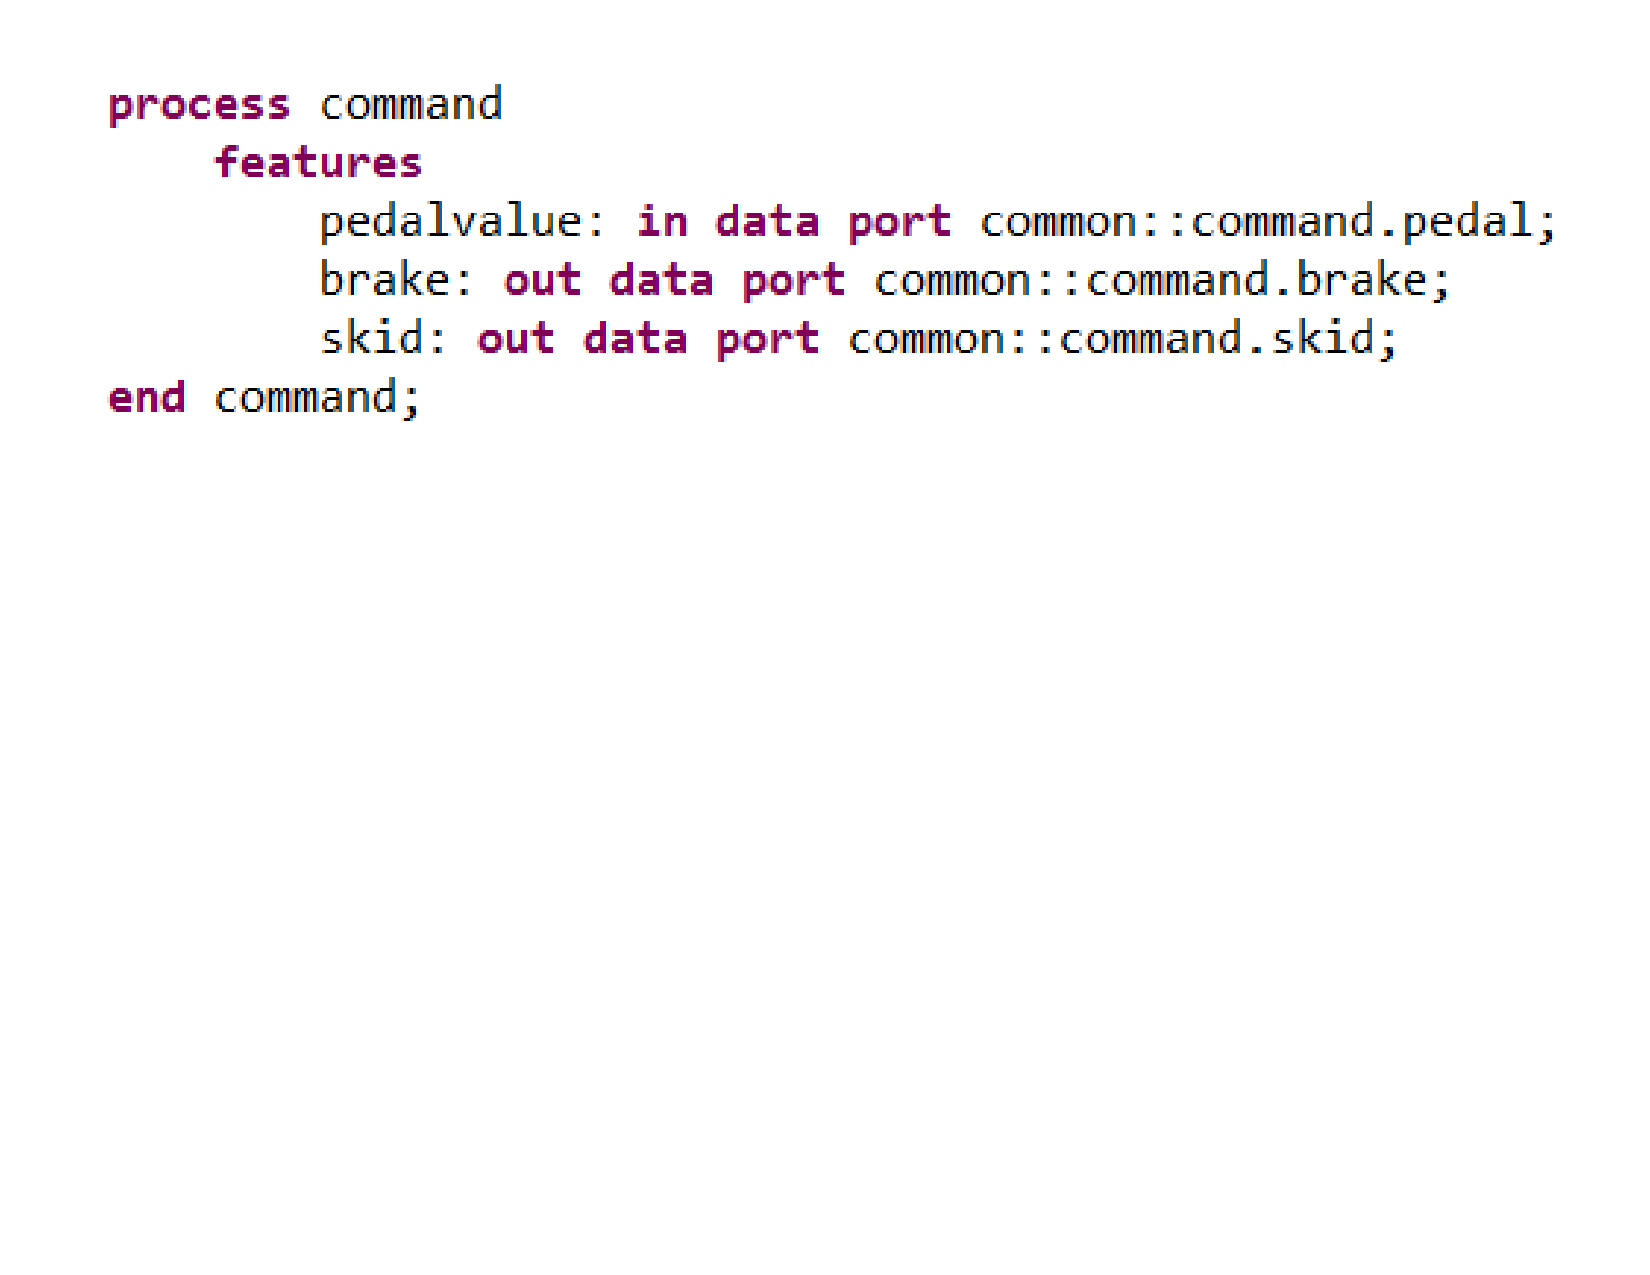
\includegraphics[clip,width=1.1\textwidth]{images/bscu_cmd_comp.pdf}
	%\vspace{-0.19in}
	\end{center}
\vspace{-0.4in}
\end{figure}

As seen in the EMV2 example, the error propagations are specified for the input and output signals, and the component error behavior describes how the component transitions to a failed state and what output errors can be propagated in that state.

Different from EMV2, the Safety Annex approach utilizes AGREE for the nominal behavior, as well as the propagations (no matter nominal or faulty). Therefore, error propagations are specified for the output signals in the Safety Annex; no error propagations for the input signals need to be explicitly specified. Furthermore, all error behaviors have to be concretely represented in terms of how they affect the output data flow, so that they can be analyzed by the back-end analysis engine. For example, adding the {\em service\_mode} element to the {\em pedalvalue} output signal of the {\em pedal} component in AADL to model the ``No Service'' error, and adding the {\em presence} element to the {\em skid} and {\em brake} output signals of the {\em command} component in AADL to model the ``No Value'' error.

Below shows an example in AGREE capturing the relationship between the {\em service\_mode} element of the {\em pedalvalue} input signal and the {\em presence} element of the {\em skid} and {\em brake} output signals:

\begin{figure}[h!]
	\hspace*{-4cm}
	\vspace{-0.3in} 
	\begin{center}
		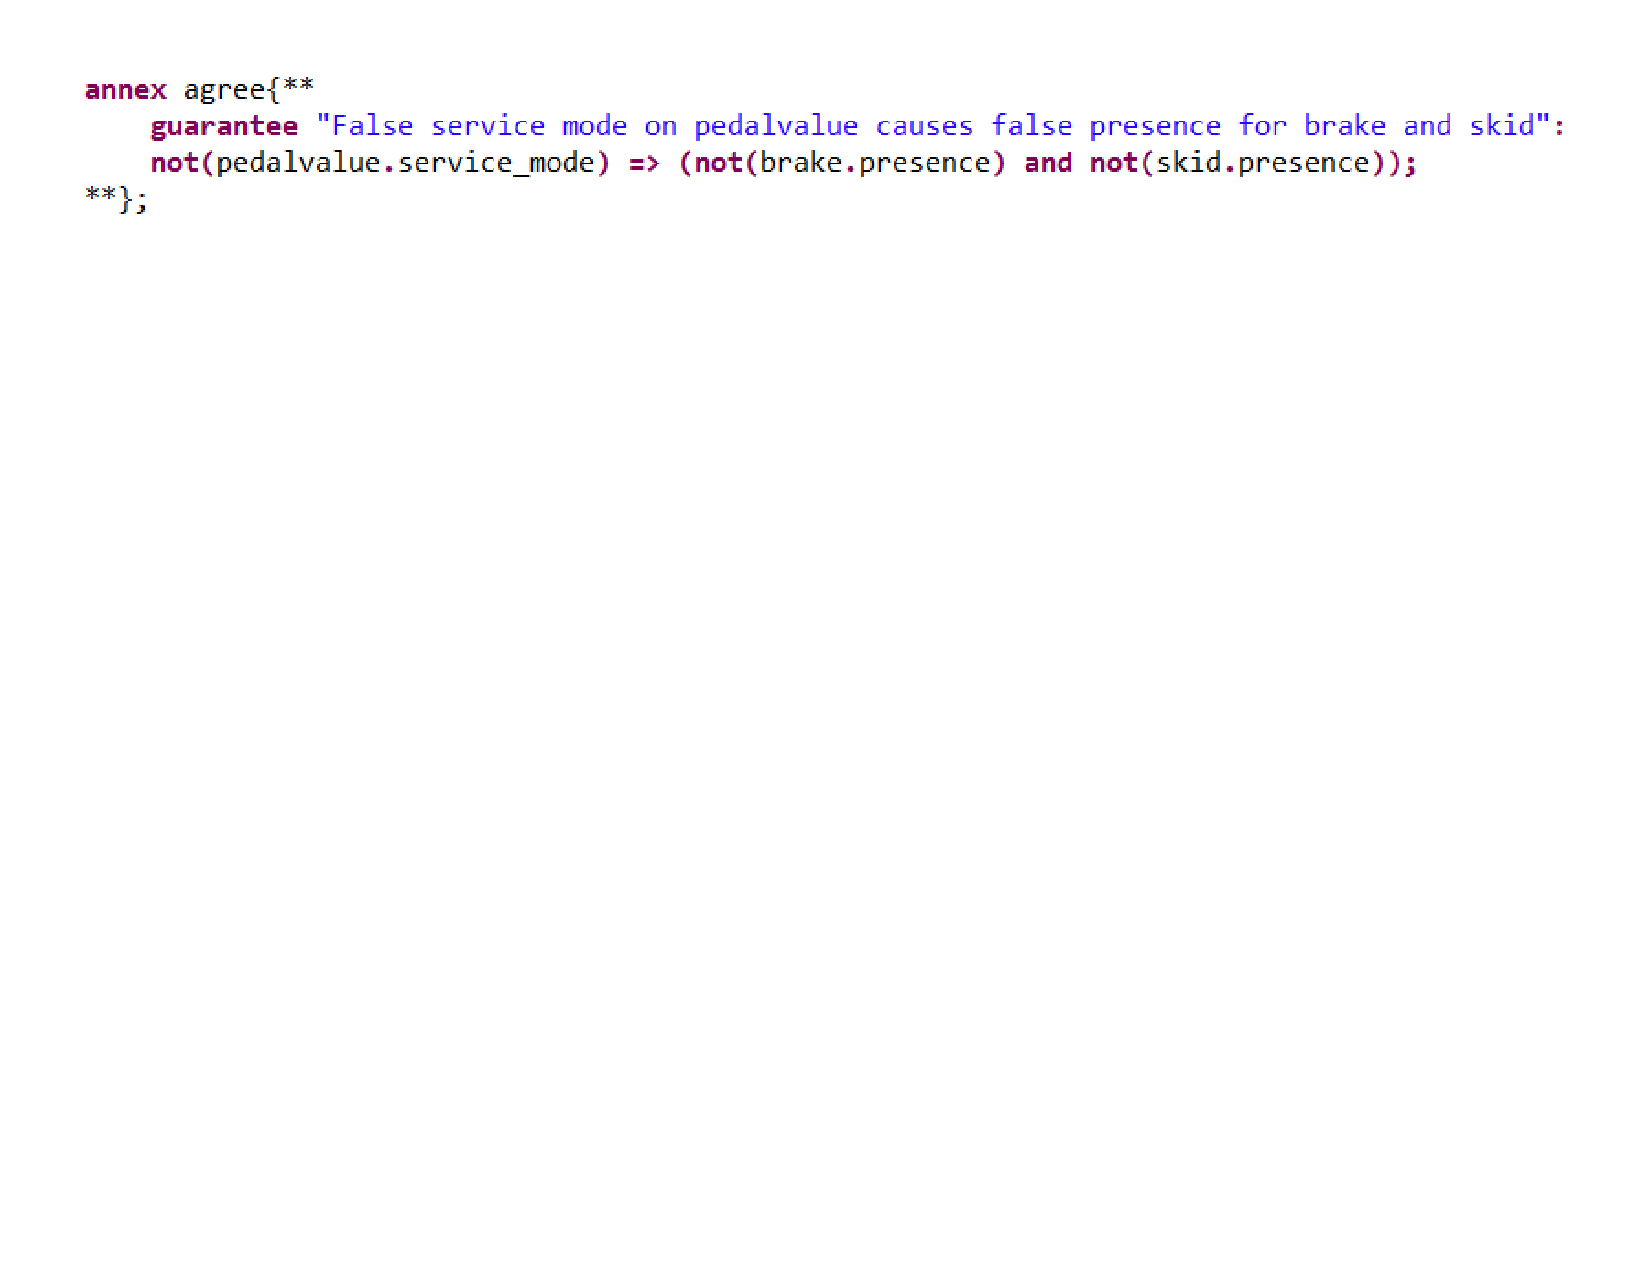
\includegraphics[width=1.0\textwidth]{images/cmd_input_agree.pdf}
		%\vspace{-0.19in}
	\end{center}
	\vspace{-3.3in}
\end{figure}






 


